% Template for PLoS
% Version 3.5 March 2018
%
% % % % % % % % % % % % % % % % % % % % % %
%
% -- IMPORTANT NOTE
%
% This template contains comments intended 
% to minimize problems and delays during our production 
% process. Please follow the template instructions
% whenever possible.
%
% % % % % % % % % % % % % % % % % % % % % % % 
%
% Once your paper is accepted for publication, 
% PLEASE REMOVE ALL TRACKED CHANGES in this file 
% and leave only the final text of your manuscript. 
% PLOS recommends the use of latexdiff to track changes during review, as this will help to maintain a clean tex file.
% Visit https://www.ctan.org/pkg/latexdiff?lang=en for info or contact us at latex@plos.org.
%
%
% There are no restrictions on package use within the LaTeX files except that 
% no packages listed in the template may be deleted.
%
% Please do not include colors or graphics in the text.
%
% The manuscript LaTeX source should be contained within a single file (do not use \input, \externaldocument, or similar commands).
%
% % % % % % % % % % % % % % % % % % % % % % %
%
% -- FIGURES AND TABLES
%
% Please include tables/figure captions directly after the paragraph where they are first cited in the text.
%
% DO NOT INCLUDE GRAPHICS IN YOUR MANUSCRIPT
% - Figures should be uploaded separately from your manuscript file. 
% - Figures generated using LaTeX should be extracted and removed from the PDF before submission. 
% - Figures containing multiple panels/subfigures must be combined into one image file before submission.
% For figure citations, please use "Fig" instead of "Figure".
% See http://journals.plos.org/plosone/s/figures for PLOS figure guidelines.
%
% Tables should be cell-based and may not contain:
% - spacing/line breaks within cells to alter layout or alignment
% - do not nest tabular environments (no tabular environments within tabular environments)
% - no graphics or colored text (cell background color/shading OK)
% See http://journals.plos.org/plosone/s/tables for table guidelines.
%
% For tables that exceed the width of the text column, use the adjustwidth environment as illustrated in the example table in text below.
%
% % % % % % % % % % % % % % % % % % % % % % % %
%
% -- EQUATIONS, MATH SYMBOLS, SUBSCRIPTS, AND SUPERSCRIPTS
%
% IMPORTANT
% Below are a few tips to help format your equations and other special characters according to our specifications. For more tips to help reduce the possibility of formatting errors during conversion, please see our LaTeX guidelines at http://journals.plos.org/plosone/s/latex
%
% For inline equations, please be sure to include all portions of an equation in the math environment.  For example, x$^2$ is incorrect; this should be formatted as $x^2$ (or $\mathrm{x}^2$ if the romanized font is desired).
%
% Do not include text that is not math in the math environment. For example, CO2 should be written as CO\textsubscript{2} instead of CO$_2$.
%
% Please add line breaks to long display equations when possible in order to fit size of the column. 
%
% For inline equations, please do not include punctuation (commas, etc) within the math environment unless this is part of the equation.
%
% When adding superscript or subscripts outside of brackets/braces, please group using {}.  For example, change "[U(D,E,\gamma)]^2" to "{[U(D,E,\gamma)]}^2". 
%
% Do not use \cal for caligraphic font.  Instead, use \mathcal{}
%
% % % % % % % % % % % % % % % % % % % % % % % % 
%
% Please contact latex@plos.org with any questions.
%
% % % % % % % % % % % % % % % % % % % % % % % %

\documentclass[10pt,letterpaper]{article}
\usepackage[top=0.85in,left=2.75in,footskip=0.75in]{geometry}

% amsmath and amssymb packages, useful for mathematical formulas and symbols
\usepackage{amsmath,amssymb}

% Use adjustwidth environment to exceed column width (see example table in text)
\usepackage{changepage}

% Use Unicode characters when possible
\usepackage[utf8x]{inputenc}

% textcomp package and marvosym package for additional characters
\usepackage{textcomp,marvosym}

% cite package, to clean up citations in the main text. Do not remove.
\usepackage{cite}

% Use nameref to cite supporting information files (see Supporting Information section for more info)
\usepackage{nameref,hyperref}

% line numbers
\usepackage[right]{lineno}

% ligatures disabled
\usepackage{microtype}
\DisableLigatures[f]{encoding = *, family = * }

% color can be used to apply background shading to table cells only
\usepackage[table]{xcolor}

% array package and thick rules for tables
\usepackage{array}

% create "+" rule type for thick vertical lines
\newcolumntype{+}{!{\vrule width 2pt}}

% create \thickcline for thick horizontal lines of variable length
\newlength\savedwidth
\newcommand\thickcline[1]{%
\noalign{\global\savedwidth\arrayrulewidth\global\arrayrulewidth 2pt}%
\cline{#1}%
\noalign{\vskip\arrayrulewidth}%
\noalign{\global\arrayrulewidth\savedwidth}%
}

% \thickhline command for thick horizontal lines that span the table
\newcommand\thickhline{\noalign{\global\savedwidth\arrayrulewidth\global\arrayrulewidth 2pt}%
\hline
\noalign{\global\arrayrulewidth\savedwidth}}


% Remove comment for double spacing
%\usepackage{setspace} 
%\doublespacing

% Text layout
\raggedright
\setlength{\parindent}{0.5cm}
\textwidth 5.25in 
\textheight 8.75in

% Bold the 'Figure #' in the caption and separate it from the title/caption with a period
% Captions will be left justified
\usepackage[aboveskip=1pt,labelfont=bf,labelsep=period,justification=raggedright,singlelinecheck=off]{caption}
\renewcommand{\figurename}{Fig}

% Use the PLoS provided BiBTeX style
\bibliographystyle{plos2015}

% Remove brackets from numbering in List of References
\makeatletter
\renewcommand{\@biblabel}[1]{\quad#1.}
\makeatother



% Header and Footer with logo
\usepackage{lastpage,fancyhdr,graphicx}
\usepackage{epstopdf}
%\pagestyle{myheadings}
\pagestyle{fancy}
\fancyhf{}
%\setlength{\headheight}{27.023pt}
%\lhead{\includegraphics[width=2.0in]{PLOS-submission.eps}}
\rfoot{\thepage/\pageref{LastPage}}
\renewcommand{\headrulewidth}{0pt}
\renewcommand{\footrule}{\hrule height 2pt \vspace{2mm}}
\fancyheadoffset[L]{2.25in}
\fancyfootoffset[L]{2.25in}
\lfoot{\today}

%% Include all macros below

\usepackage{refcount}
\usepackage{textgreek}
\usepackage{bm}

\newcommand{\unit}[1]{\,\mathrm{#1}}
\newcommand{\n}[1]{\mathrm{#1}}
\newcommand{\dd}[2]{\frac{\mathrm{d} #1}{\mathrm{d} #2}}
\newcommand*{\defeq}{\mathrel{\vcenter{\baselineskip0.5ex \lineskiplimit0pt
			\hbox{\scriptsize.}\hbox{\scriptsize.}}}%
	=}
\newcommand\subref[2]{%
	\def\myref{\getrefnumber{#1}}% extract the reference number
	\hyperref[#1]{\myref\mbox{#2}}% print the reference number with argument
}

\hyphenation{XapA}
\hyphenation{XapB}
\hyphenation{XapR}
\hyphenation{XapAB}
\hyphenation{XapABR}
\hyphenation{xapA}
\hyphenation{xapB}
\hyphenation{xapR}
\hyphenation{xapAB}
\hyphenation{xapABR}

\usepackage[obeyFinal]{todonotes} % todo notes and missing figures
\reversemarginpar

%% END MACROS SECTION


\begin{document}
\vspace*{0.2in}

% Title must be 250 characters or less.
\begin{flushleft}
	{\Large
		\textbf\newline{Theoretical investigation of a genetic switch for metabolic adaptation} % Please use "sentence case" for title and headings (capitalize only the first word in a title (or heading), the first word in a subtitle (or subheading), and any proper nouns).
	}
	\newline
	% Insert author names, affiliations and corresponding author email (do not include titles, positions, or degrees).
	\\
	Kathrin Laxhauber\textsuperscript{1},
	Muir J. Morrison\textsuperscript{2},
	Rob Phillips\textsuperscript{2,3$\ast$}
	\\
	\bigskip
	\textbf{1} Dept???, ETHZ, Zurich, State???, Switzerland\todo{MJM: Add dept \& complete affiliation}
	\\
	\textbf{2} Department of Physics, California Institute of Technology, Pasadena, CA, USA
	\\
	\textbf{3} Department of Biology and Biological Engineering, California Institute of Technology, Pasadena, CA, USA
	\\
	\bigskip
	
	% Insert additional author notes using the symbols described below. Insert symbol callouts after author names as necessary.
	% 
	% Remove or comment out the author notes below if they aren't used.
	%
	% Primary Equal Contribution Note
	% Yinyang These authors contributed equally to this work.
	
	% Additional Equal Contribution Note
	% Also use this double-dagger symbol for special authorship notes, such as senior authorship.
	% \ddag These authors also contributed equally to this work.
	
	% Current address notes
	% \textcurrency Current Address: Dept/Program/Center, Institution Name, City, State, Country % change symbol to "\textcurrency a" if more than one current address note
	% \textcurrency b Insert second current address 
	% \textcurrency c Insert third current address
	
	% Use the asterisk to denote corresponding authorship and provide email address in note below.
	$\ast$ phillips@pboc.caltech.edu
	
\end{flushleft}
% Please keep the abstract below 300 words
\section*{Abstract}
Membrane transporters carry important molecules through the cell membrane
and, from a resource standpoint, should only be produced when necessary. The
expression of membrane transporters in metabolic pathways is often
upregulated by the transporter substrate. In \emph{E. coli}, such systems
include for example the \emph{lacY}, \emph{araFGH}, and \emph{xylFGH} genes,
which encode for lactose, arabinose, and xylose transporters, respectively.
As a case study, we build a physical model of the \emph{xapABR} genetic
circuit, which features a regulatory feedback loop through membrane
transport (positive feedback) and enzymatic degradation (negative feedback)
of an inducer. Dynamical systems analysis and stochastic simulations show
that the membrane transport makes the model system bistable in certain
parameter regimes. Thus, it serves as a genetic “on-off” switch, enabling
the system to only produce a set of metabolic enzymes when the corresponding
metabolite is present in large amounts. We find that the negative feedback
from the degradation enzyme does not significantly disturb the positive
feedback from the membrane transporter. We investigate hysteresis in the
switching and discuss the role of cooperativity and multiple binding sites
in the model circuit. Altogether, this work explores how a stable genetic
switch for a set of enzymes is obtained from transcriptional auto-activation
of a membrane transporter through its substrate.

\linenumbers

% Use "Eq" instead of "Equation" for equation citations.
% For figure citations, please use "Fig" instead of "Figure".
% Place figure captions after the first paragraph in which they are cited.
% Results and Discussion can be combined.
% Place tables after the first paragraph in which they are cited.
% PLOS does not support heading levels beyond the 3rd (no 4th level headings).
% Include only the SI item label in the paragraph heading. Use the \nameref{label} command to cite SI items in the text.

\section*{Introduction}
Genetic regulatory circuits are fundamental building blocks of functioning
cells and organisms. One abundant class of these circuits are genetic
switches. Although their construction and function may differ,
their common feature is bistability: their output gene expression
will flow to and remain at one of two steady-state levels.
The distribution of
gene expression in a cell culture can then be bimodal. This is not to be
confused with mere stochastic bimodality, where the system is not stable,
and the gene expression in each cell can fluctuate between the two levels.

One classic example of a genetic switch is a system where two repressor
proteins each regulate the transcription of the
other~\cite{Jacob1961,Gardner2000} (illustrated schematically in
Fig~\ref{fig1:switches}). Here, one stable state is high expression of
the first protein and low expression of the second,
and the second stable state is the opposite. This
switch enables the system to have a memory: if something induces expression
of either one of the proteins, the system will remain in this state until a
significant perturbation occurs. Another well known and even simpler example
is an auto-activating circuit in which a protein activates its own
transcription~\cite{Wolf1998}. This gives the system an ``on-off'' switch.

\begin{figure}%[h!]
	\centering
	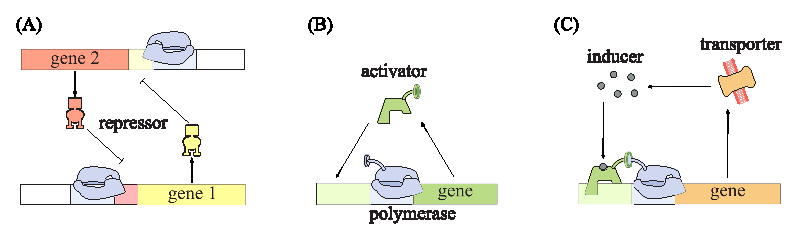
\includegraphics{media/Circuits.eps}
	\caption{{\bf A schematic of different genetic switches.}
	(A) and (B) show the two most well-known genetic switches:
	(A) two mutual repressors and (B) a self-activating gene.
	In (C), a very much simplified version of the
	circuit that we investigate in this paper can be seen, where the
	similarity to the switch in (B) becomes obvious. A complete version of
	the model circuit can be found in Fig~\ref{fig2:model}.}
	\label{fig1:switches}
\end{figure}

Through physical and mathematical modeling, we investigate a more complex
but common switch system where the bistability is due, as we will show, to a
membrane transport protein. Its key feature is the indirect activation of
the transporter gene by the transporter substrate, leading to positive
feedback similar to the aforementioned ``on-off'' switch. An example for
such an architecture is the \emph{lac} operon, where lactose indirectly
activates the expression of lactose permease. Other examples in \emph{E.
coli} include the \emph{araFGH} and \emph{xylFGH} operons, which contain genes for
arabinose and xylose transporters, respectively. For \emph{lac} and
\emph{araFGH}, bistability has indeed been observed and attributed to such a
positive feedback
loop~\cite{Novick1957,Narang2008,Choi2008,Ozbudak2004,Fritz2014,Jenkins2017,Siegele1997}.
A eukaryotic example is the glucose transporter GLUT-2 in liver and
\textbeta-cells~\cite{Bae2010,Tiedge1991}, though this system is much more
complex than the following analysis. 

It is quite conceivable that this auto-activation process is common to many
substances that a cell would want to accumulate. Such a switch enables the
cell to sense and respond to its environment: if the substrate enters the
cell, it activates the production of membrane transporters. The cell then
starts accumulating the substrate, thereby ``testing'' the substrate's
presence in the extracellular environment. If there is enough, the
expression stabilizes at an ``on'' point and the cell has, in a short-term
sense, adapted. When there is not enough substrate anymore, the operon, which
often encodes for a whole set of enzymes for this one metabolite, switches
``off'' again. Such a mechanism could be involved in various cases of
short-term adaptation.

A key element of this mechanism is the presence of a transcription factor
which is always expressed at a low level (often at copy numbers
of order $\sim10$) and which binds to the transporter substrate.
This is resource efficient for the cell, as this low copy number
transcription factor acts as an ``always on'' sensor to detect
the substrate, allowing high copy numbers of the membrane transporter
and its attendant operon to be expressed only when
their substrate is actually present. The transcription factors
LacI, AraC, and XylR all appear to fill this
role~\cite{Novick1957,Narang2008,Choi2008,Ozbudak2004,Fritz2014,Jenkins2017,Siegele1997}.
\todo{do we have a cite for xylR too?}

For our modeling, we focus on the \emph{xapABR} genetic circuit from
\emph{E. coli} as a case study. It is similar to \emph{lac}, but less
complex. Instead of lactose, its purpose is to make use of the nucleoside
xanthosine as an energy source~\cite{Buxton1980,Hammer-Jespersen1980}. The
circuit is made up of two operons: one that encodes for XapR and another
that encodes for XapA and XapB. XapR appears to be a transcription factor
that is induced by xanthosine and activates the \emph{xapAB} promoter,
in close analogy to LacI, AraC, and XylR.
The \textit{xapAB} promoter has been suggested to have two binding sites for XapR\cite{Seeger1995},
but the promoter architecture and function is not yet fully understood. The
transcription of \emph{xapR} seems to be constitutive and not
auto-regulated~\cite{Seeger1995}. Structural homology to other transcription
factors suggests that XapR appears in dimers where one dimer can bind two
xanthosine molecules~\cite{Joergensen1999}. The protein XapA is a purine
nucleoside phosphorylase that degrades xanthosine into components (ribose
and xanthine) that can be fed into metabolic
pathways~\cite{Buxton1980,Hammer-Jespersen1980}. XapB on the other hand is a
membrane transporter of xanthosine~\cite{Seeger1995,Norholm2001}.

Experimentally it was found that the expression level of \emph{xapAB} among
cells follows a bimodal distribution and that the system seems to be
bistable~\cite{Chure2019}. We aim to understand which of the circuit's
features are necessary for bistability and investigate its behavior in
different parameter regimes. In the following section, we will discuss the
details of our model. After estimating the free parameters we then present
the observations we made through phase diagrams, followed by the results
from stochastic simulations.


\section*{Model}
\subsection*{Step by step modeling of the system}
In this section, we present our model of the \emph{xapAB} genetic circuit.
Fig~\ref{fig2:model} shows an overview of this model. It consists of the
following steps: 
\begin{itemize}
	\item Small amounts of xanthosine are transported into and out of cell in various ways (discussed in more detail later on).
	\item XapR is induced by xanthosine.
	\item The induced XapR binds to the \emph{xapAB} promoter, leading to transcription.
	\item From this mRNA transcript, translation produces the two proteins XapA and XapB.
	\item XapB actively transports much larger amounts of xanthosine into the cell and XapA degrades xanthosine.
	\item At some point, the proteins decay.
\end{itemize}
Because xanthosine induces the transcription factor XapR, we have a positive
and negative feedback loop due to XapB and XapA, respectively. The remainder
of this subsection discusses each of the above steps in detail, leading us
to a set of two coupled ODE's. More in-depth explanations can be found
in~\nameref{S1_Text}.

\begin{figure}[h!]
	\centering
	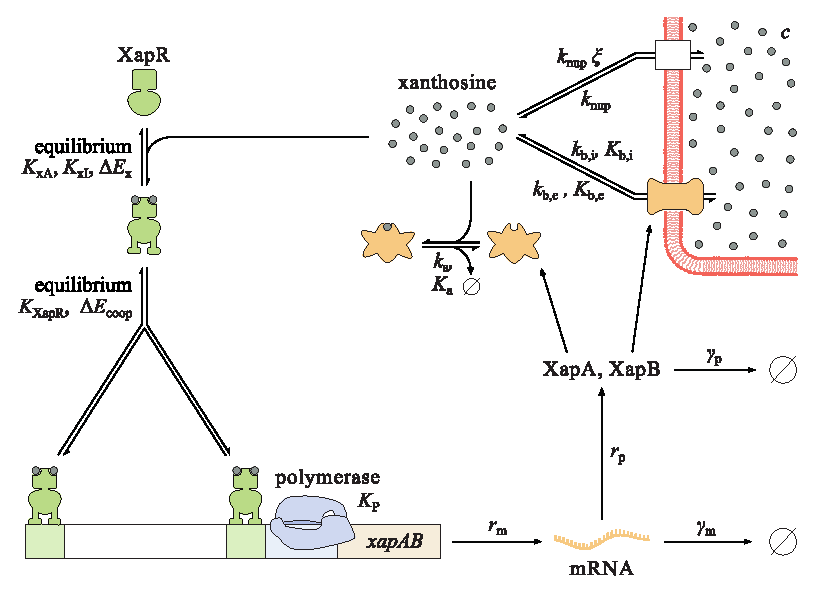
\includegraphics{media/XapSystem.eps}
	\caption{{\bf Model of the \emph{xapAB} circuit.}
		The XapR dimers are induced by xanthosine and the induced XapR binds
		cooperatively as an activator to the \emph{xapAB} promoter. For
		these two steps, quasi-equilibrium is assumed. If both XapR binding
		sites are occupied and the polymerase is bound, the gene is
		transcribed at rate $r_{\n{m}}$. The mRNA decays at rate
		$\gamma_{\n{m}}$, and both proteins are translated at rate
		$r_{\n{p}}$ and decay at rate $\gamma_{\n{p}}$. XapA degrades
		xanthosine with Michaelis-Menten parameters $k_{a}$ and $K_a$.
		Similarly, XapB imports and exports xanthosine with parameters
		$k_{\n{b,i}}, K_{\n{b,i}}$ and $k_{\n{b,e}}, K_{\n{b,e}}$,
		respectively. Furthermore, xanthosine enters and leaves the cell in
		other ways, proportional to rates $k_{\n{nup}}$ and $\xi
		k_{\n{nup}}$, respectively.}
	\label{fig2:model}
\end{figure}

\paragraph*{Induction of XapR.} 
We treat dimers as the only form of XapR that appears in the cell. Each
dimer can bind two xanthosine molecules. The Monod-Wyman-Changeux (MWC)
model is used to describe the fraction of XapR dimers in the active state: 
\begin{eqnarray}
\label{eq:MWC}
\n{[XapR]_A} = \n{[XapR]_{tot}} \frac{\left(1 + \frac{\n{[x]}}{K_{\n{xA}}}\right)^2}{\left(1 + \frac{\n{[x]}}{K_{\n{xA}}}\right)^2 + e^{\beta \Delta E_{\n{x}}} \left(1+\frac{\n{[x]}}{K_{\n{xA}}} \frac{K_{\n{xA}}}{K_{\n{xI}}}\right)^2}
\end{eqnarray}
Here, $\n{[x]}$ is the xanthosine concentration, and $\n{[XapR]_A}$ and
$\n{[XapR]_{tot}}$ denote the concentration of active and total XapR dimers,
respectively. Furthermore, $K_{\n{xI}}$ and $K_{\n{xA}}$ are the
dissociation constants of xanthosine to the inactive and the active XapR
dimer, respectively, and $\Delta E_{\n{x}}$ stands for the energy difference
between the inactive and the active state. We expect $\Delta E_{\n{x}} > 0$
and $K_{\n{xA}} < K_{\n{xI}}$ for inducible activation. This corresponds to
XapR being mainly inactive in the absence of xanthosine and becoming mostly
active at high concentrations of xanthosine. A detailed discussion of the
MWC model can be found in~\cite{Marzen2013}.

\paragraph*{Transcription.} 
Transcription and translation of the \emph{xapAB} gene, regulated by the
induced XapR, produce the two proteins XapA and XapB. We start with
transcription and assume that the binding of XapR and polymerase to the
promoter is at quasi-equilibrium. The polymerase binding is modeled as
independent of that of XapR, and all influence of the activator is pushed
into the transcription rate. Furthermore, the binding energy of XapR to each
of its two sites is assumed to be the same. A discussion of these
simplifications can be found in~\nameref{S1_Text}.

In Fig~\ref{fig3:states}, all possible states of the promoter in our model
and their corresponding thermodynamic weights are shown. There, $\n{[P]}$
denotes the polymerase concentration and $\Delta E_{\n{coop}}$ stands for
the interaction energy of the two XapR dimers. If cooperativity in
transcription factor binding is neglected, this is set to zero. Furthermore,
$K_{\n{XapR}}$ and $K_{\n{P}}$ denote the dissociation constant of XapR and
polymerase to the promoter, respectively. In statistical mechanics language
this is equivalent to $\frac{N_{\mathrm{NS}}}{V} e^{\beta \Delta E_{i}}$
with $N_{\mathrm{NS}}$ being the number of non-specific binding sites on the
DNA, $V$ the volume of the cell, and $\Delta E_{i}$ the interaction energy
of $i=$XapR or $i=$polymerase with the promoter.

\begin{figure}%[h!]
	\centering
	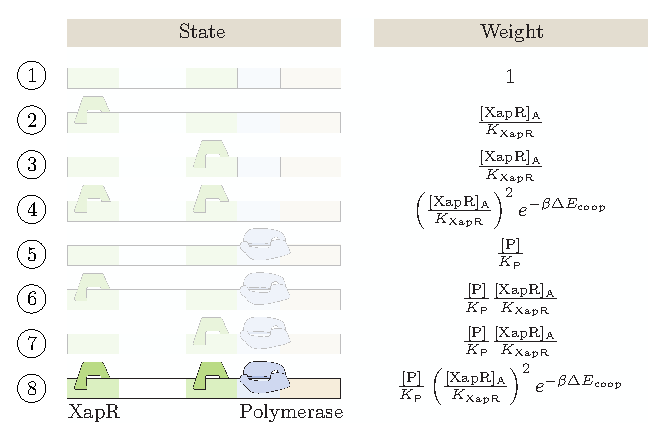
\includegraphics{media/States.eps}
	\caption{{\bf The promoter states.} We consider only the completely
	occupied state as active and all other states (faded out in the figure)
	as completely inactive. The parameters are the interaction energy of
	the two XapR dimers $\Delta E_{\n{coop}}$ and the dissociation
	constants $K_{\n{XapR}}$ and $K_{\n{P}}$ of XapR and polymerase
	to the promoter, respectively. The concentrations of polymerase
	and active XapR are denoted by $\n{[P]}$ and $\n{[XapR]}$.}
	\label{fig3:states}
\end{figure}

We consider only the state where both XapR binding sites are occupied as
active and all other states as inactive, meaning they have transcription
rate $0$. Experiments show that the expression becomes very weak when one of
the XapR binding sites is removed from the promoter, suggesting that this
simplification is reasonable~\cite{Chure2019}. Furthermore, we find that in
the bistable parameter range, considering the single occupancy states as
active instead has almost no influence on the results (see
also~\nameref{S1_Text}).

With $\n{[m]}$ being the mRNA concentration, $r_{\n{m}}$ the transcription
rate, $\gamma_{\n{m}}$ the mRNA decay rate, and $p_{\n{active}}$ the
probability of the promoter being in the active state, we obtain
\begin{eqnarray}
\label{eq:mbasic}
\dd{\n{[m]}}{t} &=& r_{\n{m}} p_{\n{active}} - \gamma_{\n{m}} \n{[m]} \\
p_{\n{active}} &=& \frac{w_8}{\sum_{i=1}^{8} w_i} = 
\frac{\n{[P]}}{K_{\n{P}}+\n{[P]}} 
\frac{
	\left( \frac{\mathrm{[XapR]_A}}{K_{\mathrm{XapR}}} \right)^2 
	e^{- \beta \Delta E_{\n{coop}}}
}{
	1 + 
	2 \frac{\mathrm{[XapR]_A}}{K_{\mathrm{XapR}}} +
	\left( \frac{\mathrm{[XapR]_A}}{K_{\mathrm{XapR}}} \right)^2 e^{- \beta \Delta E_{\n{coop}}}
}
\end{eqnarray}
Here, $w_i$ stands for the thermodynamic weight of the ith state in the
order in which they are listed in Fig~\ref{fig3:states}. As written above,
the partition function factorizes into a polymerase and a XapR term because
of our assumption of independent binding, which is further discussed
in~\nameref{S1_Text}. Note that because $r_{\n{m}}$ implicitly contains the
gene copy number per cell, it has units of $\n{M^{-1} \ s^{-1}}$ and not
just $\n{s^{-1}}$. This rate equation gives the mean mRNA concentration
$\langle\n{[mRNA]}\rangle = \frac{r_{\n{m}}}{\gamma_{\n{m}}}
p_{\n{active}}$, which we will need in the next paragraph.
In~\nameref{S1_Text}, the full chemical master equation is shown, which
leads to a Poisson distribution of the mRNA concentration with the same
mean.

\paragraph*{Translation.} 
The next step in our modeling progression is translation. As a
simplification, we write $\n{[p]}=\n{[XapA]=[XapB]}$ for the general protein
concentration. This assumes that the rates of transcription, mRNA decay,
translation, and protein decay are the same for both proteins, which, as
discussed in \nameref{S1_Text}, does not have a significant influence on the
results. We write the following rate equation for the protein concentration,
where $r_{\n{p}}$ denotes the translation rate, $\gamma_{\n{p}}$ the protein
decay rate, and $\langle \n{[mRNA]} \rangle$ the mean mRNA concentration:
\begin{eqnarray}
\label{eq:pbasic}
\dd{\n{[p]}}{t} = r_{\n{p}} \langle \n{[mRNA]} \rangle - \gamma_{\n{p}} \n{[p]}.
\end{eqnarray}

\paragraph*{Xanthosine dynamics.}
We have now discussed how xanthosine activates the synthesis of XapA and
XapB through XapR. In this part of the section, we close the feedback loop
by setting up a xanthosine rate equation. 

Transport of xanthosine across the cell membrane happens in two steps which
we will discuss now. All statements in this paragraph are based on data
from~\cite{Norholm2001}. In a first transport step, xanthosine passes the
outer membrane through porins like Tsx, OmpF and OmpC. This does not seem to
be a rate-limiting step. Then, XapB actively transports it across the inner
membrane, powered by the proton motive force. There are two other active
nucleoside transporters that seem to be transporting xanthosine with a very
low affinity: NupC and NupG. It was found that \textDelta\emph{nupC}
\textDelta\emph{nupG} strains cannot grow on xanthosine. Hence, these seem
to be necessary to ``start'' the system by importing small amounts of
xanthosine that then activate \emph{xapB}, and there appears to be no other
significant way in which xanthosine can enter the cell.

We assume the kinetic scheme of all three transporters to be similar to that
of \emph{lac} permease (as it is described in~\cite{Kaback2015}). One
transporter can then do two things to change the intracellular xanthosine
concentration $\n{[x]}$: it can actively transport one xanthosine into the
cell, powered by the proton gradient, or it can transport one out of the
cell, against the proton gradient. For net transport, a proton and a
substrate need to bind on one side of the membrane and detach from the
transporter on the other side of the membrane before the transporter goes
back to the first side again (see also~\nameref{S1_Text}). Because of the
proton gradient, influx is overall thermodynamically more likely than export
at low intracellular xanthosine concentrations, which leads to a net influx.
For much higher intra- than extracellular xanthosine concentrations, the
difference in the chemical potential of xanthosine across the membrane can
dominate that of the protons and there is net efflux. 

We model influx and efflux separately and use Michaelis-Menten kinetics for
XapB. For the turnover rate and Michaelis constant for influx we write
$k_{\n{b, i}}$ and $K_{\n{b, i}}$, respectively, and $k_{\n{b, e}}, K_{\n{b,
e}}$ for efflux. These parameters implicitly include the proton gradient.
For NupC and NupG, the Michaelis constant is very large, due to their low
xanthosine affinity. Thus, the general $k_{\n{cat}} \n{[E]_0}
\frac{\n{[S]}}{K_{\n{M}} + \n{[S]}}$ can be approximated as
$\frac{k_{\n{cat}}}{K_{\n{M}}} \n{[E]_0} \n{[S]}$. In the following,
$\frac{k_{\n{cat}}}{K_{\n{M}}} \n{[E]_0}$ is denoted by $k_{\n{nup}}$ for
influx, and the efflux rate is written as $\xi k_{\n{nup}}$. For the XapB
kinetics, no approximations can be made, because the xanthosine
concentration in the dynamic system can range from far below the respective
$K_{\n{M}}$ value to far above. The final terms for Nup and XapB are shown
below.

After transport into the cell, XapA degrades xanthosine. We model this using
standard Michaelis-Menten kinetics, with parameters $k_{\n{a}}, K_{\n{a}}$
(corresponding to turnover rate and Michaelis constant, respectively). All
the above then leads to the xanthosine rate equation
\begin{eqnarray}
\dd{\n{[x]}}{t} = \biggl(\underbrace{k_{\n{b,i}} \frac{c}{K_{\n{b,i}} + c} - k_{\n{b,e}} \frac{\n{[x]}}{K_{\n{b,e}} + \n{[x]}}}_{\n{XapB}} - \underbrace{k_{\n{a}} \frac{\n{[x]}}{K_{\n{a}} + \n{[x]}}}_{\n{XapA}}\biggr) \n{[p]} + \underbrace{k_{\n{nup}} \left(c- \xi \n{[x]}\right)}_{\n{NupC\ \& \ NupG}}.
\end{eqnarray}
We recall that $\n{[x]}$ is the intracellular xanthosine concentration, and
$c$ denotes the extracellular one. Because $k_{\n{b,i}} > k_{\n{b,e}}$ and
$K_{\n{b,i}} < K_{\n{b,e}}$, influx dominates at low intracellular
xanthosine concentrations. At much higher intra- than extracellular
xanthosine concentrations, the efflux term takes over. More details on the
aforementioned steps and a discussion of passive diffusion can be found
in~\nameref{S1_Text}.

\subsection*{Nondimensionalization}
We have now formulated the behavior of the system in terms of the rate
equations for mRNA, protein, and xanthosine. These equations can be
nondimensionalized, which reduces the dimension of parameter space. We
measure time in units of $\gamma_{\n{p}}^{-1}$ and concentrations in units
of $K_{\n{a}}$ (except XapR, where the equations make it more natural to use
$K_{\n{XapR}}$). In Table~\ref{table1:nondim}, all the nondimensional
parameters and their definitions are listed. Furthermore, we define
$\n{[m]_a} \defeq \frac{\n{[m]}}{K_{\n{a}}}$, $\n{[p]_a} \defeq
\frac{\n{[p]}}{K_{\n{a}}}$, $\n{[x]_a} \defeq \frac{\n{[x]}}{K_{\n{a}}}$,
and $\tau \defeq \gamma_{\n{p}} t$. Using these definitions, the following
equations are obtained
\begin{alignat}{2}
\dd{\mathrm{[m]_a}}{\tau} &= \ &&
\rho_{\n{m}} 
\frac{
	\mathrm{[XapR]_{R,A}}^2 
	e^{- \Delta \epsilon_{\text{coop}}}
}{
	1 + 
	2 \mathrm{[XapR]_{R,A}} +
	\mathrm{[XapR]_{R,A}}^2 e^{- \Delta \epsilon_{\text{coop}}}
}
- \gamma_{\n{mp}} \mathrm{[m]_a}
\\
\dd{\mathrm{[p]_a}}{\tau} &= \ &&
\rho_{\n{p}} \mathrm{[m]_a}
- \mathrm{[p]_a}
\\
\dd{\mathrm{[x]_a}}{\tau} &= \ && \left(k_{\n{\beta,i}} \frac{\n{[c]_a}}{K_{\n{\beta,i}} + \n{[c]_a}} - k_{\n{\beta,e}} \frac{\n{[x]_a}}{K_{\n{\beta,e}} + \n{[x]_a}} - k_{\n{\alpha}} \frac{\n{[x]_a}}{1 + \n{[x]_a}}\right) \mathrm{[p]_a} \\ & && + k_{\n{\eta}} \left(\mathrm{[c]_a} - \xi \mathrm{[x]_a}\right)
\nonumber \\
\text{with} & && \raggedleft [\n{XapR}]_{\mathrm{R,\n{A}}} = [\n{XapR}]_{\mathrm{R}} \frac{\left(1 + \frac{\mathrm{[x]_{\n{a}}}}{K_{\n{\chi A}}}\right)^2}{\left(1 + \frac{\mathrm{[x]_{\n{a}}}}{K_{\n{\chi A}}}\right)^2 + e^{\Delta \epsilon_{\n{x}}} \left(1+\frac{\mathrm{[x]_{\n{a}}}}{K_{\n{\chi A}}} \frac{1}{K_{\n{IA}}}\right)^2} \nonumber
\end{alignat}

Very little is known about the \emph{xap} system, and thus, there are no
measured values for the free parameters. Nevertheless, we were able to
estimate a reasonable range by using values from similar, well studied
systems and by finding physical constraints or relations between parameters.
The results of these estimates are shown in Table~\ref{table1:nondim}. They
are based on a choice of $\gamma_{\n{p}} = 5 \cdot 10^{-4} \unit{s^{-1}}$
and $K_{\n{a}} = 5 \cdot 10^{-5} \unit{M}$. A detailed derivation can be
found in~\nameref{S1_Text}. 

\begin{table}%[h!]
	\centering
	\caption{
		{\bf Nondimensional parameters and their estimated values.}}
	\begin{tabular}{rllr}
		\thickhline
		Param. & Definition & Estimated range & Value used \\
		\hline
		$\rho_{\n{m}}$ & $\defeq \frac{r_{\n{m}}}{\gamma_{\n{p}} K_{\n{a}}} \frac{\n{[P]}}{K_{\n{P}}+\n{[P]}}$ & $\approx 10^{-3 \pm 2}$ & $10^{-3}$ \\
		$\gamma_\n{{mp}}$ & $\defeq \frac{\gamma_{\n{m}}}{\gamma_{\n{p}}}$ & $\approx 10^{1 \pm 0.5}$ & $10^{1}$ \\
		$\rho_{\n{p}}$ & $\defeq \frac{r_{\n{p}}}{\gamma_{\n{p}}}$ & $\approx 10^{2 \pm 0.5}$ & $10^{2}$ \\
		$\n{[XapR]_R}$ & $\defeq\frac{\n{[XapR]_{\n{tot}}}}{K_{\n{XapR}}}$ & $\approx 10^{0 \pm 2}$ & $10^0$ \\
		$\n{[c]_{a}}$ & $\defeq \frac{c}{K_{\n{a}}}$ & ($\in [ 0, 10^3 ]$) & $13$ \\
		$k_{\n{\beta,i}}$ & $\defeq\frac{k_{\n{b,i}}}{\gamma_{\n{p}}}$ & $\approx 10^{4 \pm 1}$ & $5 \cdot 10^4$ \\
		$k_{\n{\beta,e}}$ & $\defeq\frac{k_{\n{b,e}}}{\gamma_{\n{p}}}$ & $\approx 10^{3 \pm 2}$ & $10^3$ \\
		$k_{\n{\alpha}}$ & $\defeq\frac{k_{\n{a}}}{\gamma_{\n{p}}}$ & $\approx 10^{2 \pm 0.8}$ & $10^2$ \\
		$k_{\n{\eta}}$ & $\defeq\frac{k_{\n{nup}}}{\gamma_{\n{p}}}$ & $\approx 10^{0 \pm 3}$ & $5 \cdot 10^{-1}$ \\
		$\xi$ & $=\xi$ & $\approx 0.8 \pm 0.1$ & $0.8$ \\
		$K_{\n{\beta,i}}$ & $\defeq\frac{K_{\n{b,i}}}{K_{\n{a}}}$ & $\approx 10^{1 \pm 2}$ & $10^1$ \\
		$K_{\n{\beta,e}}$ & $\defeq\frac{K_{\n{b,e}}}{K_{\n{a}}}$ & $\approx 10^{2 \pm 2}$ & $10^2$ \\
		$K_{\n{\chi A}}$ & $\defeq\frac{K_{\n{xA}}}{K_{\n{a}}}$ & $\approx 10^{2 \pm 1} \cdot 10^{\Delta \epsilon_{\n{x}} - 5}$ & $10^2$ \\
		$K_{\n{IA}}$ & $\defeq\frac{K_{\n{xI}}}{K_{\n{xA}}}$ & $\approx 10^{2 \pm 1}$ & $10^2$  \\
		$\Delta \epsilon_{\n{x}}$ & $\defeq\beta \Delta E_{\n{x}}$ & $\approx 2$ to $2 \left( \ln\left(K_{\n{IA}}\right) - 1\right) < 12$ & $5$ \\
		$\Delta \epsilon_{\n{coop}}$ & $\defeq \beta \Delta E_{\n{coop}}$ & $\approx 0 - 10$ & $5$ \\
		\thickhline
	\end{tabular}
	\begin{flushleft} 
		The left column shows all nondimensional parameters that appear in
		the final equations. In the middle are their definition and
		estimated values. They are based on $\gamma_{\n{p}} = 5 \cdot
		10^{-4} \unit{s^{-1}}$ and $K_{\n{a}} = 5 \cdot 10^{-5} \unit{M}$.
		Note that the range of the three MWC parameters depends on each
		other, but they can still be chosen independently. The range given
		for $\n{[c]_{a}}$ denotes the estimated ``interesting'' range in
		which switching happens, but $\n{[c]_{a}}$ can of course exceed
		these values. Details on the parameters and their estimation can be
		found in~\nameref{S1_Text}. Finally, the last column shows the value
		that we use for the rest of this paper, unless otherwise noted. An
		explanation of this choice will follow in the next section.
	\end{flushleft}
	\label{table1:nondim}
\end{table}


\section*{Results and discussion}
In the modeling process in the previous section, we have obtained three
coupled differential equations. In this section, we will analyze these
equations with deterministic methods and stochastic simulations. Analytical
closed-form solutions could not be obtained and would, if they existed,
probably not be helpful due to their large complexity. Finding such
solutions requires solving a fifth order algebraic equation.

\subsection*{Deterministic phase portraits}
A standard way to analyze dynamical systems like ours deterministically is
to plot phase portraits. In the following, we present such plots where the
state variables are the mRNA, the protein, and the xanthosine concentration.

\paragraph*{From a 3D to a 2D system.} 
Fig~\subref{fig4:bistability}{A} shows the 3D phase portrait for a
representative set of parameters (that from Table~\ref{table1:nondim}),
whose choice is explained below. The plot looks rather complicated at first
but can be understood intuitively. The three planes are the nullclines and
the gray lines point in the direction in which the dynamical system moves at
each point. The planes intersect in three points, which are the steady-state
solutions of the dynamical system. For this choice of parameters, the system
first flows towards the mRNA nullcline, then it moves along that plane to
the intersection with the protein nullcline, and lastly, it moves along that
intersection line to one of the three intersection points of all three
planes.

\begin{figure}%[h!]
	\centering
	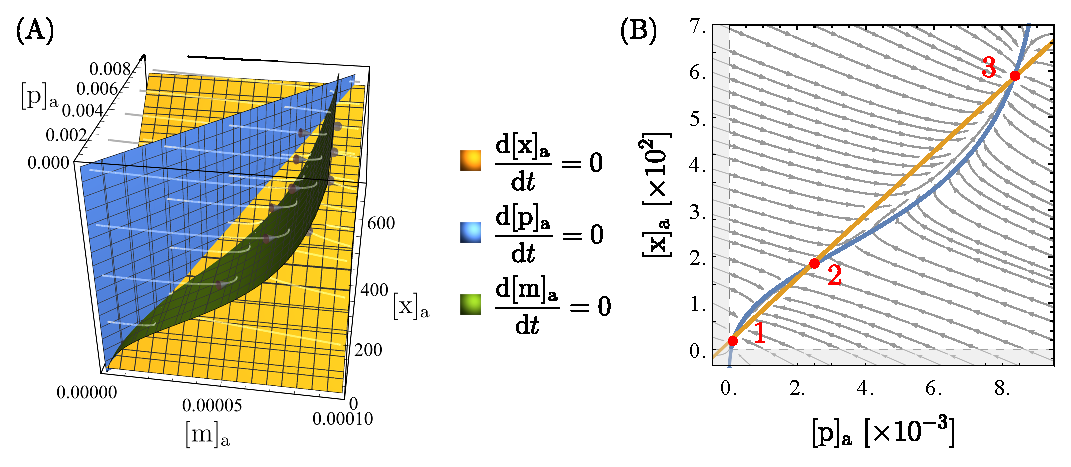
\includegraphics[width=1\textwidth]{media/Bistability.eps}
	\caption{{\bf Phase portraits showing bistability.}
		3D and 2D phase portraits for one set of parameters that leads to
		bistability. The parameter values are listed in
		Table~\ref{table1:nondim}. Note that all the concentrations
		($\n{[m]_a}, \n{[p]_a}, \n{[x]_a}$) are measured in units of
		$K_{\n{a}} = 5 \cdot 10^{4} \unit{nM}$. The planes in (A) and the
		lines in (B) are the nullclines of the state variables, and their
		intersection points, marked in red in (B), are the steady-state
		solutions of the system. The region shaded in gray in (B) leads to
		negative concentrations and is unphysical. A vector plot of (B) that
		also shows the magnitude of flow at each point can be found
		in~\nameref{S1_Text}.}
	\label{fig4:bistability}
\end{figure}
%\todo{edge,size}

It is important to point out that for a different set of parameters, the
dynamics can be quite different. There are, for example, scenarios where the
xanthosine kinetics are roughly as fast as the mRNA kinetics and the
dynamics unfolds in two steps: first to the intersection of the mRNA and the
xanthosine nullcline, then along that line to the protein nullcline and
thereby to a fixed point.

A usual simplification with genetic circuits like this is to assume the mRNA
concentration to be at steady-state, i.e. to write $\dd{\n{[m]_a}}{\tau}=0$
and solve this for $\n{[m]_a}(\n{[p]_a},\n{[x]_a})$ to simplify the 3D to a
2D system. This restricts the dynamics to the green plane in our plot, which
is reasonable here because as explained above, the system first flows
towards that plane before either the protein or the xanthosine concentration
changes significantly. However, as already pointed out, this is different
for other parameter values, and thus, this assumption generally is not a
good one. If the xanthosine dynamics are faster than the mRNA dynamics, the
system first flows towards the xanthosine nullcline. In that case, forcing
it onto the mRNA nullcline leads to significant changes in the dynamics.

Nevertheless, the steady-state solutions and the qualitative features that
we address in this paper remain the same. Because the 3D plots are rather
hard to read, we will, in the following, make the compromise to show a 2D
version of the phase portraits but ensure that all of our statements also
hold true in 3D space. As explained above, it makes the most sense here to
do this by setting $\dd{\n{[m]_a}}{\tau}=0$. The resulting equations can be
found in~\nameref{S1_Text}. In particular, we define $\rho \defeq
\frac{\rho_{\n{m}} \rho_{\n{p}}}{\gamma_{\n{mp}}}$ for everything that
follows.

\paragraph*{Bistability.} 
From the 2D plot in Fig~\subref{fig4:bistability}{B}, it can clearly be seen
that for the chosen parameters, there are three steady-state solutions.
Because the 2D plane that we are in now is the mRNA nullcline, these
solutions are the same fixed points as in the 3D plot
($\dd{\n{[m]_a}}{\tau}=0$ on the nullcline and $\dd{\n{[p]_a}}{\tau}=0$,
$\dd{\n{[x]_a}}{\tau}=0$ for the 2D fixed points). One can see from the
vector field that the two outer points (labeled 1 and 3) are stable and the
middle one (labeled 2) is unstable and serves as a sort of ``switch-point''
between the other two. This means that there are two stable states the cell
can be in, one at high (point 3) and one at low (point 1) expression. As a
result, there is bistability and the distribution of expression among cells
is bimodal.

This corresponds to the experimental observations, so the model passes this
sanity check. Furthermore, the xanthosine and protein concentrations at the
upper fixed point have the expected order of magnitude: the xanthosine
concentration is roughly $10-100 \unit{nM}$, and there are roughly $500$
proteins, which is just a bit lower than what was measured for the number of
Nup transporters~\cite{Li2014} which fulfill a similar purpose. We do not
have well founded expectations for the other fixed points, so no comparison
can be made here. Nevertheless, the orders of magnitude at the lower fixed
point -- roughly $1-10 \unit{nM}$ of xanthosine and around $5$ proteins --
seem perfectly reasonable. Note that $\n{[x]_a} \approx \n{[c]_a}$ at the
lower fixed point because there is only weak accumulation due to Nup and a
few XapB transporters.

As already mentioned, we are working with one specific set of parameters
here and we will now explain this choice of values. Firstly, they were
picked such that they are well within their estimated range. Secondly, we
wanted clear bistability to occur in the phase portraits as well as in the
stochastic simulations (see later). Thirdly, by the corresponding choice of
parameters it was ensured that the mRNA number per cell at the
``switch-point'' is around 1: this is large enough to enable the system to
clearly resolve the two stable fixed points (as we will see from the
stochastic simulations later on), but is low enough to lead to mean mRNA
numbers that are very reasonable (see~\cite{Milo2016} for the average mRNA
numbers in cells, which are rather low). The protein and xanthosine
concentrations followed from this, but with some variation in the parameters
they could still be tuned to a certain extent.

As a remark we point out that we have not observed any oscillations in the
system. Intuitively, they might be expected when the XapA rate is
significantly larger than the XapB rate, but it turns out that oscillations
cannot be obtained. This can be understood when looking at the regions that
are bounded by all three nullclines: within these regions, the streamlines
on the nullclines point into the regions, so deterministically, the system
is trapped in there and can only flow towards the fixed points.

For a different set of parameters, the orders of magnitude in the plots and
even the qualitative behavior can change. In the following, we will discuss
some interesting features of the system that can be observed through the
phase portraits. 

\paragraph*{The extracellular xanthosine concentration.}
The parameter that is the experimentally most easily tunable and
biologically the most relevant is the extracellular xanthosine
concentration. When it is increased in the experiment, the cells go from all
being in the low expression state to being in either the low or the high
expression state (all-or-none phenomenon) to all being in the high
expression state~\cite{Chure2019}. If our model is correct, it should
exhibit the same qualitative behavior. Indeed we find exactly this: as can
be seen in Fig~\ref{fig5:extraxanth}, increasing $\n{[c]_a}$ makes the high
stable fixed point appear and then, for even higher $\n{[c]_a}$, the lower
one disappear. Thus, for low $\n{[c]_a}$ the only stable point of the system
is at low expression, and for high $\n{[c]_a}$ there is only high
expression. In between, there are two deterministically stable expression
levels.

\begin{figure}%[h!]
	\centering
	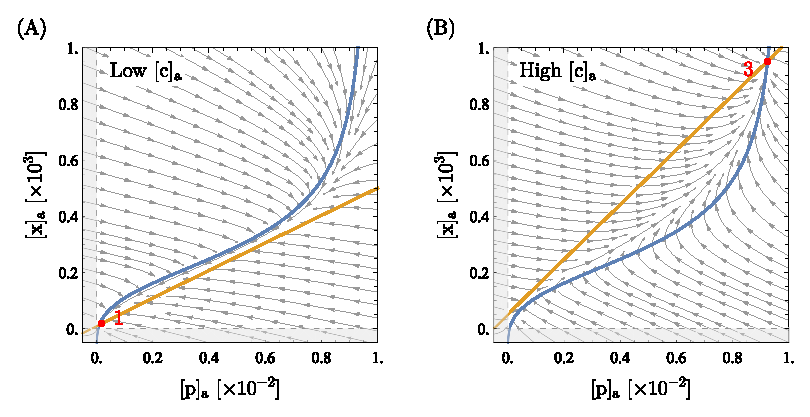
\includegraphics[width=1\textwidth]{media/VaryingC.eps}
	\caption{{\bf Phase portraits for different extracellular xanthosine concentrations.}
		All parameters but $\n{[c]_a}$ are as presented in
		Table~\ref{table1:nondim}. The extracellular xanthosine
		concentration in these plots is $\n{[c]_a}=10^{1}$ in (A) and
		$\n{[c]_a}= 5 \cdot 10^{2}$ in (B) (recall $\n{[c]_{a}} \defeq
		\frac{c}{K_{\n{a}}}$, $K_{\n{a}} = 5 \cdot 10^{-5} \unit{M}$).
		Tuning $\n{[c]_a}$ moves the orange line (xanthosine nullcline) up
		or down, the blue line (mRNA nullcline) is unchanged (see
		also~\nameref{S1_Text}). It can clearly be seen that in (A) there is
		only the lower fixed point (fixed point number 1), whereas in (B)
		there is only the upper one (fixed point number 3). In between lies
		the bistable case that was shown in Fig~\ref{fig4:bistability}.}
	\label{fig5:extraxanth}
\end{figure}
%\todo{size of plot}

Furthermore, by setting $\n{[c]_a}=0$ (not shown here) we found that in the
absence of xanthosine, there are roughly 2-3 proteins, which agrees very
well with measurements, where around 2 proteins per cell were
found~\cite{Li2014}. In addition, the parameter $K_{\n{\chi A}}$
(dissociation constant of xanthosine from active XapR) can be tuned such
that the extracellular xanthosine concentration $\n{[c]_a}$ in the
switching-regime is similar to that in the experiment. It was found that the
cell only adapts at very high xanthosine concentrations of almost a
millimolar~\cite{Norholm2001} which is not completely unexpected when
recalling that for \emph{lac}, cells also limit themselves to glucose as
long as possible. Interestingly, because there is no parameter other than
$K_{\n{\chi A}}$ that tunes the critical value of $\n{[c]_a}$, this tells us
that $K_{\n{\chi A}}$ is large as argued in the estimation of $K_{\n{\chi
A}}$ in~\nameref{S1_Text}. Thus, the interaction between xanthosine and XapR
should be weak.

\paragraph*{The roles of XapA and XapB.}
While it is clear that the bistability in the model system is due to the
feedback loop from XapA and XapB, it is not obvious if both XapA and XapB
are necessary. It turns out that the bistability is due to XapB only. XapA
is neither sufficient nor necessary and, within the estimated parameter
regime, does not even have a significant influence on the system. This can
be seen from the plots in figure~\ref{fig6:xapAB}. XapA lowers the upper
solution by a little and could, in principle, thereby make the
high-expression solution vanish. For our choice of all other parameters,
this requires $k_{\n{\alpha}} > 10^4$ which is far from what has been
measured. However, a higher rate could, in principle, be achieved by
different translation rates of XapA and XapB (see simplifications of the
model in~\nameref{S1_Text}). Hence, we cannot exclude the possibility that
XapA gets so strong that it makes bistability impossible, but this is an
extreme case. XapB, on the other hand, is essential; without it the system
only has the one fixed point at low expression.

\begin{figure}%[h!]
	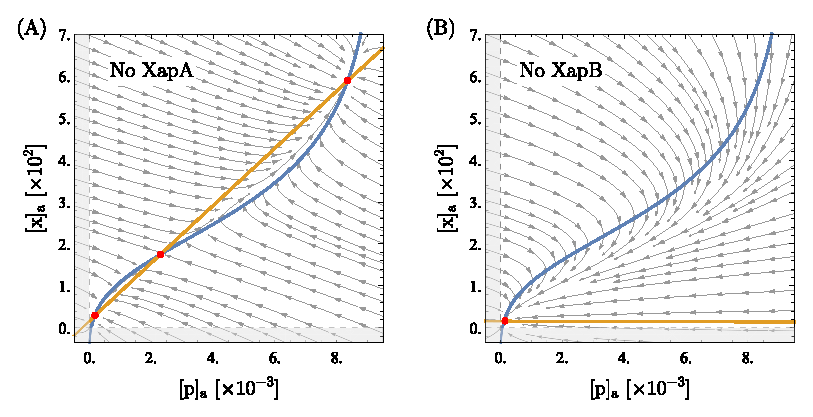
\includegraphics[width=1\textwidth]{media/XapAB.eps}
	\centering
	\caption{{\bf Phase portraits without XapA or XapB.}
		All parameters are as presented in Table~\ref{table1:nondim}. In
		(A), the XapA term was removed from the kinetic equations. In (B),
		the equations lack the two terms from XapB. These plots clearly show
		that XapA has almost no influence on the qualitative behavior of the
		system (i.e. bistability and the order of magnitudes), but XapB is
		the essential feature for bistability.}
	\label{fig6:xapAB}
\end{figure}
%\todo{size of plot}

For a cell, the above is a useful feature: by coupling XapA and XapB on an
operon, XapA is switched on and off together with XapB but it does not
significantly disturb this adaptation mechanism, while its kinetic
parameters can be chosen somewhat freely as necessary for metabolism. By
having a membrane transporter gene on an operon whose expression is
activated by the transporter substrate, the expression of a whole set of
enzymes can be turned on and off depending on the presence of the substrate.
It seems likely that this way of short-term adaptation of a single cell to
its environment may be used by cells for many metabolic processes.

\paragraph*{The role of cooperativity.} 
The model has two cooperatively interacting binding sites for XapR on the
\emph{xapAB} promoter and two cooperative binding sites on XapR for
xanthosine. An interesting question to pose is whether the cooperativity is
a necessary feature for bistability. This is motivated by the importance of
cooperativity in typical ``genetic switches''\cite{Gardner2000,Cherry2000}.

If, as a purely theoretical consideration, we remove either the second
xanthosine binding site on XapR or the second XapR binding site on the
promoter, we find that the system still has a bistable parameter regime.
However, this is only a rather narrow parameter range which makes the system
less stable. When the second binding site is removed in both places, the
equations are insufficiently non-linear to produce bistability. An example
of these three scenarios can be seen in Fig~\ref{fig7:coop}. It follows that
there need to be either two xanthosine binding sites on XapR or two XapR
binding sites on the promoter (or both) in order to obtain a switch-like
behavior. 

\begin{figure}%[h!]
	\centering
	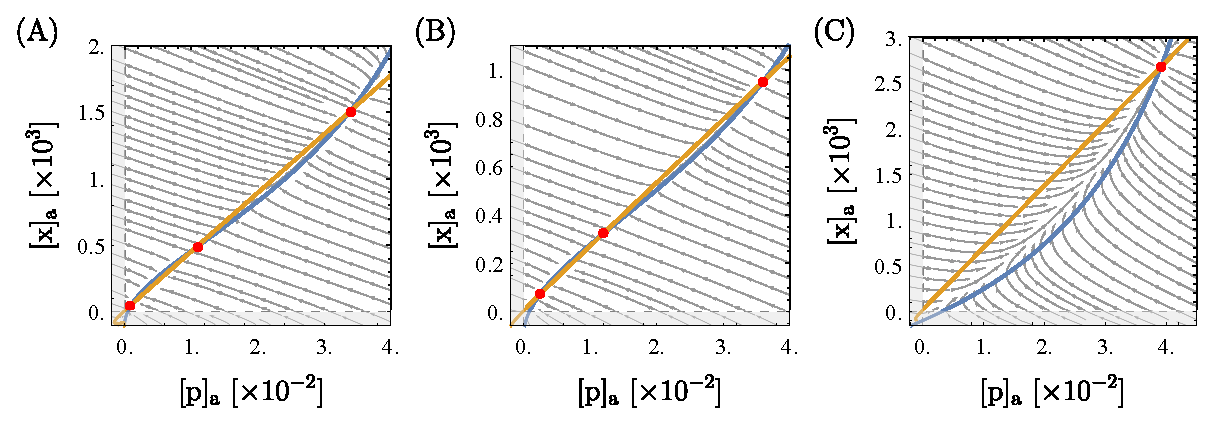
\includegraphics[width=1\textwidth]{media/FewerSites.eps}
	\caption{{\bf Phase portraits for less or no cooperativity.}
		Most parameters are as presented in Table~\ref{table1:nondim},
		changes are mentioned below. Fixed points are marked in red. In (A),
		there is only one xanthosine binding site on XapR and everything
		unchanged for the XapR-promoter binding. Two parameters are changed:
		$\rho = 0.07$ and $\n{[c]_a} = 6$. This is necessary to compensate
		for the weaker induction such that the system is bistable. In (B),
		there is only one XapR binding site on the promoter and everything
		is unchanged for the xanthosine-XapR binding. Two parameters are
		changed: $\rho = 0.13$ and $\n{[c]_a} = 3$. In (C), there is only
		one xanthosine binding site on XapR and also only one XapR binding
		site on the the promoter. Two parameters are changed: $\rho = 0.1$
		and $\n{[XapR]_R} = 5$. Whereas bistability is retained in (A) and
		(B), it cannot be obtained anymore in (C).}
	\label{fig7:coop}
\end{figure}
%\todo{size of plot}

One can also ask how much cooperative interaction is needed between the two
binding sites. For the promoter, this is given by $\Delta E_{\n{coop}}$ in
our model, and we find that setting $\Delta E_{\n{coop}} = 0$ has almost no
influence on the phase diagrams. For XapR, the two binding sites interact
indirectly, because the active state is much likelier if two xanthosine
molecules are bound. This cooperative interaction can, however, not be tuned
like in the case of the promoter with $\Delta E_{\n{coop}}$. 

Note that we are not writing Hill equations and measuring cooperativity in
terms of the Hill coefficient. If Hill equations were to be used for the
modeling, the Hill coefficient could have values between 1 and 2, which
would yield bistability for large enough values, but not for lower ones.
This could be investigated more rigorously similar to the analysis of a
simple genetic switch in~\cite{Cherry2000}. However, we refrain from looking
for a minimal Hill coefficient in our system, because we do not find this
very insightful. Hill equations only describe scenarios with multiple,
non-interacting binding sites where any other state but the fully occupied
and active or the fully empty and inactive state is not significantly
populated. In that sense, the Hill coefficient simply denotes the number of
binding sites and does not reflect how cooperative these binding sites are.
We suggest that cooperativity should be explored more in-depth and a more
rigorous analysis of the role of cooperativity in simple genetic switches
should be done before returning to more complex systems like this one.

\subsection*{Stochastic simulations}
Stochastic simulations of the full 3-dimensional system of mRNA, protein,
and xanthosine were run for comparison with the deterministic results.
In~\nameref{S1_Text}, we present the underlying chemical master equation of
the system. Because of the two different fixed points at low and high
expression, the copy numbers in the problem vary from very low to very high.
For large amounts of mRNA, protein, and xanthosine, the number of reactions
is large too, and thus, Gillespie's classical algorithm has a large
computational cost and his \texttau-leap algorithm would be ideal. On the
other hand, \texttau-leaping cannot be used for the small copy numbers. For
these reasons, we chose to work with the algorithm described
in~\cite{Cao2006}, a hybrid form between Gillespie's classical and his
\texttau-leap algorithm. We gratefully worked with the Python implementation
of this algorithm in \emph{StochPy}, version 2.3~\cite{Maarleveld2015}.

\paragraph*{Bimodality and the extracellular xanthosine concentration.}
This approach results in the same bimodal distributions that were already
seen in the deterministic investigation and experimental studies.
Fig~\ref{fig8:stochC} shows the distribution of protein expression found in
the simulations for different values of the extracellular xanthosine
concentration. The parameters that were used are the same as in the previous
section (listed in Table~\ref{table1:nondim}). To obtain the distributions,
we ran the simulation 5000 times for a simulated time of $10^6 \unit{s}$
each and started at a mRNA, protein and intracellular xanthosine count of 0.


\begin{figure}%[h!]
	\centering
	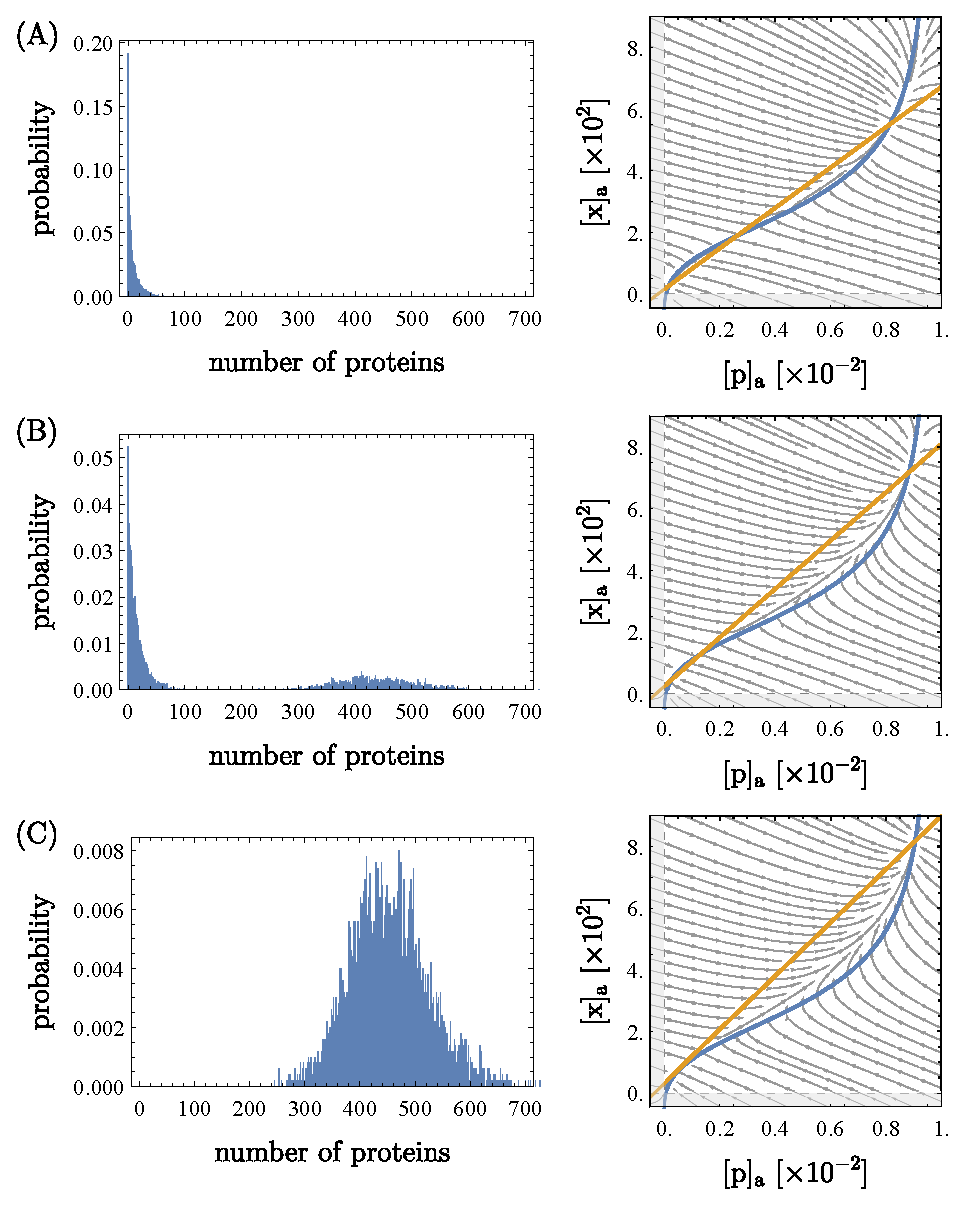
\includegraphics[width=1\textwidth]{media/HistogramsC.eps}
	\caption{{\bf Distributions from stochastic simulations and the corresponding phase portraits.}
		Apart from $\n{[c]_a}$, the parameters are the same as in
		Table~\ref{table1:nondim}. For the distributions, the simulations
		were run 5000 times for $10^6 \unit{s}$ each (simulated time) and
		started at a mRNA, protein and intracellular xanthosine count of 0.
		We show the two cases of unimodality (low expression in (A) and high
		expression in (C)) as well as the case of bimodality in (B). The
		values of $\n{[c]_a}$ are 12 in (A), 18.5 in (B), and 25 in (C)
		(recall $\n{[c]_{a}} \defeq \frac{c}{K_{\n{a}}}$, $K_{\n{a}} = 5
		\cdot 10^{-5} \unit{M}$). The output from the stochastic simulations
		is in good agreement with the concentrations at the fixed points in
		the deterministic phase portraits.}
	\label{fig8:stochC}
\end{figure}

The results agree very well with the deterministic fixed points and
experiments: the mean numbers of mRNA, protein, and xanthosine in the
stochastic results are as predicted from the phase portraits. It does,
however, become clear that the phase portraits do not tell whether the cells
will actually populate both the high and the low expression state: as can be
seen in Fig~\subref{fig8:stochC}{(A)}, the cells did not switch to the high
expression state for the waiting time in our simulations, even though one
would naively expect this from the phase portrait.

We found that the two lower fixed points (marked as 1 and 2 in
Fig~\ref{fig4:bistability}) need to be very close like in
Fig~\subref{fig8:stochC}{(B)} to give bimodality. For lower $\n{[c]_a}$,
meaning larger distance between the first and second fixed point, no or
almost no switching was observed. Of course, this is also a matter of the
waiting time and stochastic effects: if one waits for long enough, switching
should eventually occur. However, switching times of more than several hours
are not at the center of this investigation and would mean that switching is
extremely unlikely. There are two aspects that become relevant in this
context that we neglect in our analysis but shortly mention here:
transcription and translation bursts lead to higher stochasticity and cell
division leads to some discontinuity in the process.

Note that while the deterministic analysis assumes the variables to be
continuous, the simulations work with discrete numbers of mRNA, protein, and
xanthosine. This per se is no problem, because the deterministic analysis
describes the mean values and the simulation fluctuates around this mean.
If, however, the mRNA number at the third, high fixed point is too low, the
system will not be able to resolve the two points anymore. This becomes a
problem when the distance between the first and the third fixed point
becomes as low as the stochastic fluctuations in the system, which is around
3 mRNA molecules. In Fig~\ref{fig8:stochC}, the mRNA number at the low fixed
point was fluctuating between 0 and 2 with a mean significantly smaller than
1, and at the high fixed point it was varying between 2 and 6.

\paragraph*{Time evolution and switching times.}
Fig~\ref{fig:StochT} shows the time evolution of one specific example.
Again, the simulation was started with a mRNA, protein and intracellular
xanthosine count of 0 and was run for a simulated time of $5 \cdot 10^5
\unit{s}$. In this specific example, switching occurred after $10^5
\unit{s}$. 

Comparing this to the experimentally expected timescales is difficult,
because the switching time strongly depends on the extracellular xanthosine
concentration. Experiments were always stopped after a few hours, and in
this time, the cell population might not reach its steady-state expression
distribution. Hence, the distribution could be bimodal when the experiment
is stopped but become unimodal after further waiting. That way,
extracellular xanthosine concentrations that are too high for deterministic
bistability could lead to experimental bimodality if the experiment is
stopped too early. In this case, the observed switching time would be
shorter, which makes the comparison to our simulations even harder. Thus, we
cannot say if it is problematic that the $10^5 \unit{s}$ is larger than what
was found in the experiment.

Nevertheless, we do warn the reader that the timescales in the simulations
should be taken with reservations. Cell divisions are not considered here,
and neither is the burstiness of transcription and translation. This means
that stochasticity may be larger in the real system which should have an
influence on the timescales and probably shorten the time until switching
occurs.

\begin{figure}%[h!]
	\centering
	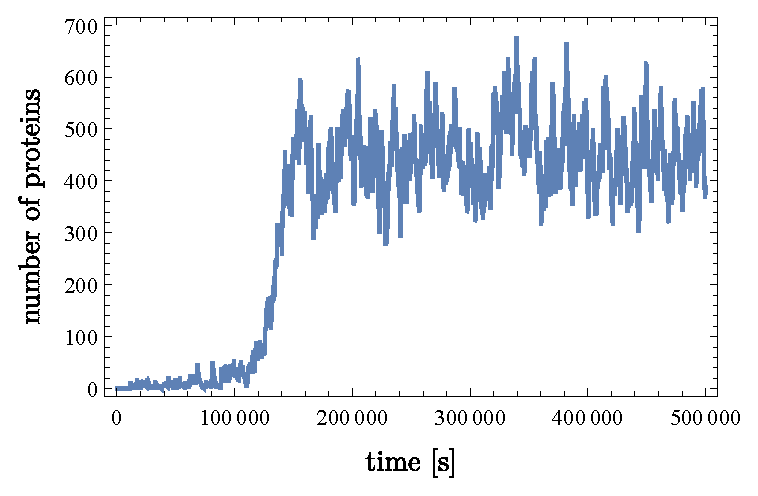
\includegraphics[width=0.7\textwidth]{media/TimeEvolution.eps}
	\caption{{\bf Time evolution of protein (XapA/XapB) from one run of the simulation.}
		The simulation was run once for $5 \cdot 10^5 \unit{s}$ and started
		at an mRNA, protein and intracellular xanthosine count of 0. In this
		case the system switched into the high-expression state after $10^5
		\unit{s}$. The parameters that were used are the same as in
		Table~\ref{table1:nondim}, the only exception being the
		extracellular xanthosine concentration, which was chosen to be
		$\n{[c]_a} = 25$ (recall $\n{[c]_{a}} \defeq \frac{c}{K_{\n{a}}}$,
		$K_{\n{a}} = 5 \cdot 10^{-5} \unit{M}$) just as in
		Fig~\subref{fig8:stochC}{(B)}.}
	\label{fig:StochT}
\end{figure}
%\todo{size of plot}

\paragraph*{Hysteresis.} 
In the previous two paragraphs, the simulations were started at initial
intracellular concentrations of 0 to investigate what happens if xanthosine
is suddenly added to the cell's environment. We can now ask the opposite
question: what happens when xanthosine is removed from the extracellular
environment? To answer this, the simulation was started with initially fully
induced cells, i.e. at the mRNA, protein and intracellular xanthosine counts
of the high fixed point in the corresponding phase portrait. 

The resulting distributions can be found in~\nameref{S1_Text}. They show
clear hysteresis effects: at concentrations where all cells remained in the
low expression state when being started there before, all cells now remain
at high expression. Only when the second and the third fixed point are very
close does switching to the uninduced state happen. Interestingly, this
behavior is symmetric to the ``switching on'' in the previous paragraphs,
where the lower two fixed points needed to be about as close as the upper
two need to be now for ``switching off''. The extracellular xanthosine
concentration (for the other parameters being as in
Table~\ref{table1:nondim}) needed to be as low as $\n{[c]_a} = 10$ to
observe bimodality and $\n{[c]_a}=9$ to have all cells in the low expression
state (recall $\n{[c]_{a}} \defeq \frac{c}{K_{\n{a}}}$, $K_{\n{a}} = 5 \cdot
10^{-5} \unit{M}$). \todo{Is this understandable without seeing the data? Do
you have any suggestions to make it clearer?}

We have learned that cells only change their metabolism to xanthosine if
enough of the latter is around, but after they have switched, this metabolic
state is stable even if the xanthosine concentration decreases to a certain
extent. This explains what has been observed by Novick and
Weiner~\cite{Novick1957} for the \emph{lac} operon: when induced cells were
transferred into lower concentrations of lactose, they remained induced,
even though uninduced cells could not become induced at these
concentrations.


\section*{Conclusion}
\paragraph*{A genetic switch for metabolic adaptation with remarkable features.}
In this paper, we propose a model for biological pathway systems containing
a membrane transporter whose gene expression is, directly or indirectly,
activated by its substrate. We have shown that such a system can be bistable
and thus work as a genetic switch which reacts to the extracellular
concentration of the relevant metabolite. This switch has very useful
biological features: first, coupling of the transporter with, for example, a
degradation enzyme creates a genetic switch that enables short-term
adaptation of the cell's metabolism to its environment. Second, the switch
is stabilized by hysteresis effects when the extracellular xanthosine
concentration decreases, which explains previous experimental findings.

\paragraph*{Required properties for this system.}
We have found that no bistability can emerge from the genetic circuit unless
at least one component has two binding sites for its activator. Additional
binding sites or cooperativity seem to increase the stability of the switch.
In addition, simply knowing the experimental switching concentration of
xanthosine let us, for example, infer the approximate value of the
dissociation constant between the transcription factor XapR and the inducer
xanthosine. We found that their interaction needs to be rather weak.

\paragraph*{Possibilities for further investigation.}
Phase diagrams, showing for which parameters the system is bistable and for
which there is only the lower or the upper stable fixed point, could be
calculated from arguments made in~\cite{Cherry2000}. However, the
simulations have shown that deterministic bistability does not mean that
bimodality occurs, which is why we have refrained from showing such
diagrams. Furthermore, the timescales in the problem could be investigated
more thoroughly, for example the dependence of the switching time on
$\n{[c]_a}$. Having said that, the simulation for such an analysis should
account for the burstiness of transcription and translation as well as for
cell divisions, which is anything but straightforward. Lastly, some rigorous
work could be done to identify the most and least relevant parameters of the
system to create a simpler, minimal model that captures the most relevant
features.

\paragraph*{General lessons learned for the modeling of other systems.}
We point out again that assuming the mRNA concentration to be at
steady-state can have a significant impact on the apparent dynamics of a
system, as we have seen in the 3-dimensional phase portraits. Moreover, we
remind the reader that deterministic phase portraits do not show which
states are actually populated, and thus hide essential effects like
hysteresis. Lastly, we have exemplified issues with the common picture of
measuring cooperativity in terms of the Hill coefficient: the Hill
coefficient simply denotes the number of binding sites and does not reflect
how cooperative these binding sites are. 

\paragraph*{A successful model.}
All model parameters could be estimated fairly well despite the lack of deep
experimental knowledge about the model system. In the results, every
variable and parameter has its expected order of magnitude, which suggests
that the model captures all relevant features and is able to describe the
dynamics of the \emph{xap} system. With the framework given in this text, it
should be straightforward to model other promoters, regulatory pathways or
enzymes and thereby adapt the model to other genes and metabolites. Examples
include \emph{lac}, \emph{ara}, and \emph{xyl}, but we suspect that many if
not most metabolic processes involve the adaptation mechanism that we have
investigated here, and that a lot can be understood about them through our
model. This apparent success demonstrates once more that even for broadly
unknown systems, rigorous physical modeling can potentially offer an
efficient way to gain a very thorough understanding of the behavior of the
system. 

\todo{Is the conclusion too long?}


\section*{Supporting information}
\paragraph*{S1 Text.}
\label{S1_Text}
{\bf The aforementioned further information.} Discussion of simplifications
in the model, parameter estimation, elaborations on the results, and the
chemical master equation of this circuit.

\section*{Acknowledgments}
We thank Griffin Chure, Charlotte Strandkvist, and Kyle Naughton for
providing their data on the \emph{xap} system and pointing out the
bistability. We also thank Griffin Chure for answering any biological
questions that arose, Nathan Belliveau for bringing similar systems to our
attention, and Jane Kondev and Jin Wang for interesting discussions. Plots
were done in \emph{Mathematica} using the packages MaTeX and
CurvesGraphics6. K.S.L. acknowledges financial support from the
Werner~Siemens-Foundation through the Swiss Study Foundation.
\todo[inline]{I don't really know what/who is usually listed here... Did I list too many people (I don't know at what ``extent'' of help people are usually named here) or did I forget anyone? Should I list everyone who worked on the xap system last summer and provided the data even though they are already cited, but only as Griffin et al.? Is it enough to list packages like this or should I try to find some website to cite? Should I list Python \& StochPy again it's already mentioned in the text? SHould I thank someone for the providing the elements for the figures and whom? Is there funding that should be listed?}

\nolinenumbers

% Either type in your references using
% \begin{thebibliography}{}
% \bibitem{}
% Text
% \end{thebibliography}
%
% or
%
% Compile your BiBTeX database using our plos2015.bst
% style file and paste the contents of your .bbl file
% here. See http://journals.plos.org/plosone/s/latex for 
% step-by-step instructions.
 	
\begin{thebibliography}{10}
	
	\bibitem{Jacob1961}
	Jacob F, Monod J.
	\newblock Genetic regulatory mechanisms in the synthesis of proteins.
	\newblock Journal of Molecular Biology. 1961;3(3):318--356.
	
	\bibitem{Gardner2000}
	Gardner TS, Cantor CR, Collins JJ.
	\newblock Construction of a genetic toggle switch in \emph{Escherichia coli}.
	\newblock Nature. 2000;403:339.
	
	\bibitem{Wolf1998}
	Wolf DM, Eeckman FH.
	\newblock On the Relationship between Genomic Regulatory Element Organization
	and Gene Regulatory Dynamics.
	\newblock Journal of Theoretical Biology. 1998;195(2):167 -- 186.
	\newblock doi:{https://doi.org/10.1006/jtbi.1998.0790}.
	
	\bibitem{Novick1957}
	Novick A, Weiner M.
	\newblock Enzyme induction as an all-or-none phenomenon.
	\newblock Proceedings of the National Academy of Sciences of the United States
	of America. 1957;43(16590055):553--566.
	
	\bibitem{Narang2008}
	Narang A, Pilyugin SS.
	\newblock Bistability of the lac Operon During Growth of Escherichia coli on
	Lactose and Lactose + Glucose.
	\newblock Bulletin of Mathematical Biology. 2008;70(4):1032--1064.
	
	\bibitem{Choi2008}
	Choi PJ, Cai L, Frieda K, Xie XS.
	\newblock A Stochastic Single-Molecule Event Triggers Phenotype Switching of a
	Bacterial Cell.
	\newblock Science. 2008;322(5900):442--446.
	\newblock doi:{10.1126/science.1161427}.
	
	\bibitem{Ozbudak2004}
	Ozbudak EM, Thattai M, Lim HN, Shraiman BI, van Oudenaarden A.
	\newblock Multistability in the lactose utilization network of
	\emph{Escherichia coli}.
	\newblock Nature. 2004;427:737.
	
	\bibitem{Fritz2014}
	Fritz G, Megerle JA, Westermayer SA, Brick D, Heermann R, Jung K, et~al.
	\newblock Single Cell Kinetics of Phenotypic Switching in the Arabinose
	Utilization System of E. coli.
	\newblock PLOS ONE. 2014;9(2):e89532.
	\newblock doi:{10.1371/journal.pone.0089532}.
	
	\bibitem{Jenkins2017}
	Jenkins A, Macauley M.
	\newblock Bistability and Asynchrony in a Boolean Model of the l-arabinose
	Operon in Escherichia coli.
	\newblock Bulletin of Mathematical Biology. 2017;79(8):1778--1795.
	
	\bibitem{Siegele1997}
	Siegele DA, Hu JC.
	\newblock Gene expression from plasmids containing the araBAD promoter at
	subsaturating inducer concentrations represents mixed populations.
	\newblock Proceedings of the National Academy of Sciences of the United States
	of America. 1997;94(9223333):8168--8172.
	
	\bibitem{Bae2010}
	Bae JS, Kim TH, Kim MY, Park JM, Ahn YH.
	\newblock Transcriptional Regulation of Glucose Sensors in Pancreatic
	beta-Cells and Liver: An Update.
	\newblock Sensors. 2010;10(5):5031–5053.
	\newblock doi:{10.3390/s100505031}.
	
	\bibitem{Tiedge1991}
	Tiedge M, Lenzen S.
	\newblock Regulation of glucokinase and GLUT-2 glucose-transporter gene
	expression in pancreatic beta-cells.
	\newblock The Biochemical journal. 1991;279 (Pt 3)(1953686):899--901.
	
	\bibitem{Buxton1980}
	Buxton RS, Hammer-Jespersen K, Valentin-Hansen P.
	\newblock A second purine nucleoside phosphorylase in \emph{Escherichia coli}
	K-12.
	\newblock Molecular and General Genetics MGG. 1980;179(2):331--340.
	
	\bibitem{Hammer-Jespersen1980}
	Hammer-Jespersen K, Buxton RS, Hansen TD.
	\newblock A second purine nucleoside phosphorylase in \emph{Escherichia coli}
	K-12.
	\newblock Molecular and General Genetics MGG. 1980;179(2):341--348.
	
	\bibitem{Seeger1995}
	Seeger C, Poulsen C, Dandanell G.
	\newblock Identification and characterization of genes (xapA, xapB, and xapR)
	involved in xanthosine catabolism in \emph{Escherichia coli}.
	\newblock Journal of bacteriology. 1995;177(7559336):5506--5516.
	
	\bibitem{Joergensen1999}
	Jorgensen C, Dandanell G.
	\newblock Isolation and characterization of mutations in the \emph{Escherichia
		coli} regulatory protein XapR.
	\newblock Journal of bacteriology. 1999;181(10400599):4397--4403.
	
	\bibitem{Norholm2001}
	Norholm MH, Dandanell G.
	\newblock Specificity and topology of the \emph{Escherichia coli} xanthosine
	permease, a representative of the NHS subfamily of the major facilitator
	superfamily.
	\newblock Journal of bacteriology. 2001;183(11466294):4900--4904.
	
	\bibitem{Chure2019}
	Chure G, et~al.
	\newblock Measurements on the \emph{xapABR} system in \emph{E. coli.};
	Unpublished.
	
	\bibitem{Marzen2013}
	Marzen S, Garcia HG, Phillips R.
	\newblock Statistical Mechanics of Monod--Wyman--Changeux (MWC) Models.
	\newblock Journal of Molecular Biology. 2013;425(9):1433 -- 1460.
	\newblock doi:{https://doi.org/10.1016/j.jmb.2013.03.013}.
	
	\bibitem{Kaback2015}
	Kaback HR.
	\newblock A chemiosmotic mechanism of symport.
	\newblock Proceedings of the National Academy of Sciences.
	2015;112(5):1259--1264.
	\newblock doi:{10.1073/pnas.1419325112}.
	
	\bibitem{Li2014}
	Li GW, Burkhardt D, Gross C, Weissman J.
	\newblock Quantifying Absolute Protein Synthesis Rates Reveals Principles
	Underlying Allocation of Cellular Resources.
	\newblock Cell. 2014;157(3):624 -- 635.
	\newblock doi:{https://doi.org/10.1016/j.cell.2014.02.033}.
	
	\bibitem{Milo2016}
	Milo R, Phillips R.
	\newblock In: Cell biology by the numbers. Garland Science. 2016; 217.
	
	\bibitem{Cherry2000}
	Cherry JL, Adler FR.
	\newblock How to make a Biological Switch.
	\newblock Journal of Theoretical Biology. 2000;203(2):117--133.
	
	\bibitem{Cao2006}
	Cao Y, Gillespie DT, Petzold LR.
	\newblock Efficient step size selection for the tau-leaping simulation method.
	\newblock J Chem Phys. 2006;124(4):044109.
	\newblock doi:{10.1063/1.2159468}.
	
	\bibitem{Maarleveld2015}
	Maarleveld TR, Olivier BG, Bruggeman FJ. StochPy, Stochastic Modeling in
	Python. 2015.
	\newblock Available from: \url{http://stochpy.sourceforge.net/}.
	
\end{thebibliography}

\todo[inline]{Should I also list the references that are cited in the appendix?}

\todo[inline]{The capitalization style is different for the titles of the references. Should I list them as they are on the corresponding paper or should I do it uniformly? Does it matter at all? Otherwise I leave it as it is.}

\end{document}

